% Preamble
% Compile with XeLateX

\documentclass[11pt,oneside,a4paper,titlepage]{article}
\usepackage{preamble}
\graphicspath{{PIC/}}
%%%%%%%%%%%%%%%%%%%%%%%%%%%%%%%%%%%%%%%%%%%%%%%%%%%%%%%%%%%%%%%%%%%%%%%%%%%%%%%%%%%%%%
\begin{document}

\sidebar{sideBarColor!25}
\simpleheader{titleBackColor}{Huw Coverdale}{Jones}{Technical Writer}{white}

% Start Minipages
\vspace*{3.49cm}% start 8 cm from the top of the page}
    \adjustbox{valign=t}{\begin{minipage}{7.3cm} % large 7.4 cm from the top
    \scriptsize
    \vspace*{1.2cm} % text starts 1cm under the top of the minipage
            
        % Picture
        \begin{center}
        \begin{tikzpicture}
            \node[
            circle,
            minimum size=\cvPictureWidth,
            path picture={
            \node at (path picture bounding box.center){
             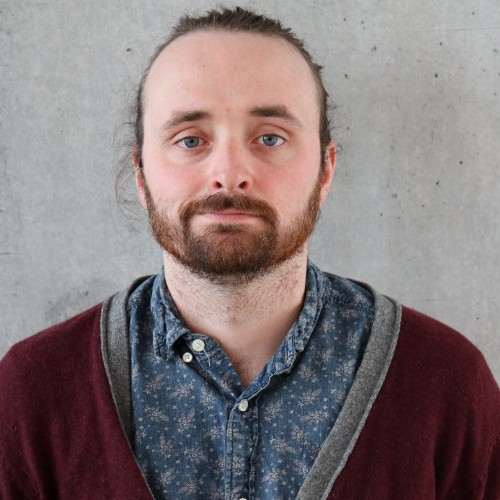
\includegraphics[width=\cvPictureWidth]{huw.jpeg}
             };
             }]
            {};
        \end{tikzpicture}
        \end{center}

       
        % Contact Section
        \begin{spacing}{1.5}
        \ruleline{\textbf{Contact}}
        \begin{tikzpicture}[every node/.style={inner sep=0pt, outer sep=0pt}]
        \matrix [
        column 1/.style={anchor=center,contactIcon},
        column 2/.style={anchor=west,align=left,contactIcon},
        column sep=5pt,
        row sep=5pt] (contact) {
        
        \node{\faEnvelope}; 
         & \node{\href{mailto:huwcoverdalejones@gmail.com}{huwcoverdalejones@gmail.com}};\\
       
        \node{\faPhone}; 
         & \node{+354 784-1195};\\ 
        \node{\faMapMarker}; 
        & \node{Seltjarnarnes, Iceland};\\
        \node{\faLinkedinSquare}; 
        & \node{\href{https://www.linkedin.com/in/huw-jones-9541b147/}{huw-jones9541b147}};\\
       } ;
        \end{tikzpicture} 
        
        %%%%%%%%%%%%%%%%%%%%%%%%%%%%%%%%%%%%%%%%%%%%%%%%%%%
        \ruleline{\textbf{Languages}}
        \begin{tikzpicture}[every node/.style={inner sep=0pt, outer sep=0pt}]
        \matrix [
        column 1/.style={anchor=center,contactIcon},
        column 2/.style={anchor=west,align=left,contactIcon},
        column sep=5pt,
        row sep=5pt] (contact) {
        \node{\flag{England.png}};
        & \node{English - Native Languages};\\
        \node{\flag{southk.jpg}};
        & \node{Korean - Professional Conversational Fluency};\\
        \node{\flag{china.png}};
        & \node{Chinese - Professional Conversational Fluency};\\
        \node{\flag{iceland.jpg}};
        & \node{Icelandic - Passed Citizenship Test August 2022};\\
        };
        \end{tikzpicture} 

        \ruleline{\textbf{Technical Skills}}
        \begin{tikzpicture}[every node/.style={inner sep=0pt, outer sep=0pt}]
        \matrix [
        column 1/.style={anchor=center,contactIcon},
        column 2/.style={anchor=west,align=left,contactIcon},
        column sep=5pt,
        row sep=5pt] (contact) {

        \node{\flag{asciidoc.png}};
        & \node{Asciidoc - Long Time Competent User};\\
        \node{\flag{latex.png}};
        & \node{LaTex - Long Time Competent User};\\
        \node{\flag{markdown.png}};
        & \node{Markdown - Long Time Competent User};\\
        \node{\flag{git.png}};
        & \node{Git - General Competency for Version Management};\\
        \node{\flag{dita.png}};
        & \node{DITA-XML - Basic Understanding for Documentation};\\
        \node{\flag{tux.png}};
        & \node{Linux Mint and Ubuntu- Keen user since Ubuntu 11.10};\\
        \node{\flag{tux.png}};
        & \node{USB Linux- Keen USB distribution user: Tails OS, MX etc.};\\
        };
        \end{tikzpicture}

        \ruleline{\textbf{Profile}}
        \begin{tikzpicture}[every node/.style={inner sep=0pt, outer sep=0pt}]
        \matrix [
        column 1/.style={anchor=center,contactIcon},
        column 2/.style={anchor=west,align=left,contactIcon},
        column sep=5pt,
        row sep=5pt] (contact) {

        \node{\flag{travels.png}};
        & \node{British/Irish Citizen - Can work in EU and UK Legally.};\\
        \node{\flag{travels.png}};
        & \node{Well Travelled - Lived in Taiwan, Korea, and China.};\\
        \node{\flag{mic.png}};
        & \node{Stand Up Comedian - Performed \& written since 2012.};\\
        \node{\flag{Gym.png}};
        & \node{Exercise - Regularly lift free weights and do yoga.};\\
        };
        \end{tikzpicture}
         \end{spacing}
    \end{minipage}} %
    \hfill 
%%%%%%%%%%%%%%%%%%%%%%%%%%%%%%%%%%%%%%%%%%%%%%%%%%%%%%%%%
%%%%% MAIN SECTION %%%%%%%%%%%%%%%%%%%%
    \adjustbox{valign=t}{\begin{minipage}{11.3cm}
    
        \vspace*{1.5cm}
        \section*{  {\faGraduationCap} Education}
        
        \MySection{2015 - 2017}{}{University of Iceland}{MSc Environment and Natural Resources - Renewable Energy
        }{Reykjavik, Iceland}{Awarded by Faculty of Industrial Engineering, Mechanical Engineering and Computer Science}{\\\textbf{Grade: 7.5}}
            
        \vspace*{0.12cm}
        
        \MySection{2014}{}
        {School of Oriental and African Studies}
        {Certificate in Teaching English for Academic Purposes}{London, UK}{Professional Qualification in Teaching English for Higher Education Students.}{\\
        \textbf{Grade: Pass}}

        \vspace*{0.12cm}

        \MySection{2012}{}{Highbury College}{CELTA}{Portsmouth, UK}{Certificate in English Language Teaching to Adults.}{\\
        \textbf{Grade: Pass}}

        \vspace*{0.12cm}
            
        \MySection{2007-2012}{}{School of Oriental and African Studies}{BA Chinese and Korean}{London, UK}{In depth language degree in Chinese and Korean, including studies in Beijing and Seoul.}{\\
        \textbf{Grade: 2:1}}

        \vspace*{0.3cm}
        %%%%%%%%%%%%%%%%%%%%%%%%%%%%%%%%%%%%%%%%%%%%%%%%%%%
        % Work Experience
        \section*{{\faSuitcase} Work Experience}
            
        \MySectionNoPic{2021-2023}{Technical Writer}{Kopavogur, Iceland}
        {Tern Systems}
        {\begin{itemize} \scriptsize
            \item Authored, reviewed, and edited technical documentation on all Tern Pojects.
            \item Spearheaded conversion process documents to create a cohesive pdf output.
            \item Created documentation templates for all documents.
            \item Oversaw documents in Office tools, specifically Google Docs, and code Formats, primarily Asciidoc.
            \item Learned Asciidoc, Markdown, LaTeX, and DITA-XML for the role. 
        \end{itemize}}  
        
        \vspace*{0.12cm}
            
        \MySectionNoPic{2019-2021}{DPM Technician}{Reyjavik, Iceland}{Alvotech}
        {\begin{itemize} \scriptsize
            \item Carried out general clinical manufacturing duties in a Pharmaceutical GMP workplace. 
            \item Developed technical knowledge of clinical manufacturing tools, including Autoclave and VHP Chamber. \item Updated process documentation, including SOPs.
        \end{itemize}}
        
        \vspace*{0.12cm}
        
        \MySectionNoPic{2017-2019}{Process Engineer}{Reyjavik, Iceland}{Omega Algae}
        {\begin{itemize} \scriptsize
            \item Planned and built plumbing solutions for the algae reactor systems. 
            \item Monitored, maintained, and repaired of electrical systems, sensors, and pumps. 
            \item Wrote and updated technical documentation, both SOPs, and experimental data reports.
            \item Used and maintained centrifuge, with focus on  cleaning, repair, and diagnostics.
        \end{itemize}}
    \end{minipage}} %




\end{document}
